% Options for packages loaded elsewhere
% Options for packages loaded elsewhere
\PassOptionsToPackage{unicode}{hyperref}
\PassOptionsToPackage{hyphens}{url}
\PassOptionsToPackage{dvipsnames,svgnames,x11names}{xcolor}
%
\documentclass[
  letterpaper,
  DIV=11,
  numbers=noendperiod]{scrartcl}
\usepackage{xcolor}
\usepackage{amsmath,amssymb}
\setcounter{secnumdepth}{-\maxdimen} % remove section numbering
\usepackage{iftex}
\ifPDFTeX
  \usepackage[T1]{fontenc}
  \usepackage[utf8]{inputenc}
  \usepackage{textcomp} % provide euro and other symbols
\else % if luatex or xetex
  \usepackage{unicode-math} % this also loads fontspec
  \defaultfontfeatures{Scale=MatchLowercase}
  \defaultfontfeatures[\rmfamily]{Ligatures=TeX,Scale=1}
\fi
\usepackage{lmodern}
\ifPDFTeX\else
  % xetex/luatex font selection
\fi
% Use upquote if available, for straight quotes in verbatim environments
\IfFileExists{upquote.sty}{\usepackage{upquote}}{}
\IfFileExists{microtype.sty}{% use microtype if available
  \usepackage[]{microtype}
  \UseMicrotypeSet[protrusion]{basicmath} % disable protrusion for tt fonts
}{}
\makeatletter
\@ifundefined{KOMAClassName}{% if non-KOMA class
  \IfFileExists{parskip.sty}{%
    \usepackage{parskip}
  }{% else
    \setlength{\parindent}{0pt}
    \setlength{\parskip}{6pt plus 2pt minus 1pt}}
}{% if KOMA class
  \KOMAoptions{parskip=half}}
\makeatother
% Make \paragraph and \subparagraph free-standing
\makeatletter
\ifx\paragraph\undefined\else
  \let\oldparagraph\paragraph
  \renewcommand{\paragraph}{
    \@ifstar
      \xxxParagraphStar
      \xxxParagraphNoStar
  }
  \newcommand{\xxxParagraphStar}[1]{\oldparagraph*{#1}\mbox{}}
  \newcommand{\xxxParagraphNoStar}[1]{\oldparagraph{#1}\mbox{}}
\fi
\ifx\subparagraph\undefined\else
  \let\oldsubparagraph\subparagraph
  \renewcommand{\subparagraph}{
    \@ifstar
      \xxxSubParagraphStar
      \xxxSubParagraphNoStar
  }
  \newcommand{\xxxSubParagraphStar}[1]{\oldsubparagraph*{#1}\mbox{}}
  \newcommand{\xxxSubParagraphNoStar}[1]{\oldsubparagraph{#1}\mbox{}}
\fi
\makeatother

\usepackage{color}
\usepackage{fancyvrb}
\newcommand{\VerbBar}{|}
\newcommand{\VERB}{\Verb[commandchars=\\\{\}]}
\DefineVerbatimEnvironment{Highlighting}{Verbatim}{commandchars=\\\{\}}
% Add ',fontsize=\small' for more characters per line
\usepackage{framed}
\definecolor{shadecolor}{RGB}{241,243,245}
\newenvironment{Shaded}{\begin{snugshade}}{\end{snugshade}}
\newcommand{\AlertTok}[1]{\textcolor[rgb]{0.68,0.00,0.00}{#1}}
\newcommand{\AnnotationTok}[1]{\textcolor[rgb]{0.37,0.37,0.37}{#1}}
\newcommand{\AttributeTok}[1]{\textcolor[rgb]{0.40,0.45,0.13}{#1}}
\newcommand{\BaseNTok}[1]{\textcolor[rgb]{0.68,0.00,0.00}{#1}}
\newcommand{\BuiltInTok}[1]{\textcolor[rgb]{0.00,0.23,0.31}{#1}}
\newcommand{\CharTok}[1]{\textcolor[rgb]{0.13,0.47,0.30}{#1}}
\newcommand{\CommentTok}[1]{\textcolor[rgb]{0.37,0.37,0.37}{#1}}
\newcommand{\CommentVarTok}[1]{\textcolor[rgb]{0.37,0.37,0.37}{\textit{#1}}}
\newcommand{\ConstantTok}[1]{\textcolor[rgb]{0.56,0.35,0.01}{#1}}
\newcommand{\ControlFlowTok}[1]{\textcolor[rgb]{0.00,0.23,0.31}{\textbf{#1}}}
\newcommand{\DataTypeTok}[1]{\textcolor[rgb]{0.68,0.00,0.00}{#1}}
\newcommand{\DecValTok}[1]{\textcolor[rgb]{0.68,0.00,0.00}{#1}}
\newcommand{\DocumentationTok}[1]{\textcolor[rgb]{0.37,0.37,0.37}{\textit{#1}}}
\newcommand{\ErrorTok}[1]{\textcolor[rgb]{0.68,0.00,0.00}{#1}}
\newcommand{\ExtensionTok}[1]{\textcolor[rgb]{0.00,0.23,0.31}{#1}}
\newcommand{\FloatTok}[1]{\textcolor[rgb]{0.68,0.00,0.00}{#1}}
\newcommand{\FunctionTok}[1]{\textcolor[rgb]{0.28,0.35,0.67}{#1}}
\newcommand{\ImportTok}[1]{\textcolor[rgb]{0.00,0.46,0.62}{#1}}
\newcommand{\InformationTok}[1]{\textcolor[rgb]{0.37,0.37,0.37}{#1}}
\newcommand{\KeywordTok}[1]{\textcolor[rgb]{0.00,0.23,0.31}{\textbf{#1}}}
\newcommand{\NormalTok}[1]{\textcolor[rgb]{0.00,0.23,0.31}{#1}}
\newcommand{\OperatorTok}[1]{\textcolor[rgb]{0.37,0.37,0.37}{#1}}
\newcommand{\OtherTok}[1]{\textcolor[rgb]{0.00,0.23,0.31}{#1}}
\newcommand{\PreprocessorTok}[1]{\textcolor[rgb]{0.68,0.00,0.00}{#1}}
\newcommand{\RegionMarkerTok}[1]{\textcolor[rgb]{0.00,0.23,0.31}{#1}}
\newcommand{\SpecialCharTok}[1]{\textcolor[rgb]{0.37,0.37,0.37}{#1}}
\newcommand{\SpecialStringTok}[1]{\textcolor[rgb]{0.13,0.47,0.30}{#1}}
\newcommand{\StringTok}[1]{\textcolor[rgb]{0.13,0.47,0.30}{#1}}
\newcommand{\VariableTok}[1]{\textcolor[rgb]{0.07,0.07,0.07}{#1}}
\newcommand{\VerbatimStringTok}[1]{\textcolor[rgb]{0.13,0.47,0.30}{#1}}
\newcommand{\WarningTok}[1]{\textcolor[rgb]{0.37,0.37,0.37}{\textit{#1}}}

\usepackage{longtable,booktabs,array}
\usepackage{calc} % for calculating minipage widths
% Correct order of tables after \paragraph or \subparagraph
\usepackage{etoolbox}
\makeatletter
\patchcmd\longtable{\par}{\if@noskipsec\mbox{}\fi\par}{}{}
\makeatother
% Allow footnotes in longtable head/foot
\IfFileExists{footnotehyper.sty}{\usepackage{footnotehyper}}{\usepackage{footnote}}
\makesavenoteenv{longtable}
\usepackage{graphicx}
\makeatletter
\newsavebox\pandoc@box
\newcommand*\pandocbounded[1]{% scales image to fit in text height/width
  \sbox\pandoc@box{#1}%
  \Gscale@div\@tempa{\textheight}{\dimexpr\ht\pandoc@box+\dp\pandoc@box\relax}%
  \Gscale@div\@tempb{\linewidth}{\wd\pandoc@box}%
  \ifdim\@tempb\p@<\@tempa\p@\let\@tempa\@tempb\fi% select the smaller of both
  \ifdim\@tempa\p@<\p@\scalebox{\@tempa}{\usebox\pandoc@box}%
  \else\usebox{\pandoc@box}%
  \fi%
}
% Set default figure placement to htbp
\def\fps@figure{htbp}
\makeatother





\setlength{\emergencystretch}{3em} % prevent overfull lines

\providecommand{\tightlist}{%
  \setlength{\itemsep}{0pt}\setlength{\parskip}{0pt}}



 


\KOMAoption{captions}{tableheading}
\makeatletter
\@ifpackageloaded{tcolorbox}{}{\usepackage[skins,breakable]{tcolorbox}}
\@ifpackageloaded{fontawesome5}{}{\usepackage{fontawesome5}}
\definecolor{quarto-callout-color}{HTML}{909090}
\definecolor{quarto-callout-note-color}{HTML}{0758E5}
\definecolor{quarto-callout-important-color}{HTML}{CC1914}
\definecolor{quarto-callout-warning-color}{HTML}{EB9113}
\definecolor{quarto-callout-tip-color}{HTML}{00A047}
\definecolor{quarto-callout-caution-color}{HTML}{FC5300}
\definecolor{quarto-callout-color-frame}{HTML}{acacac}
\definecolor{quarto-callout-note-color-frame}{HTML}{4582ec}
\definecolor{quarto-callout-important-color-frame}{HTML}{d9534f}
\definecolor{quarto-callout-warning-color-frame}{HTML}{f0ad4e}
\definecolor{quarto-callout-tip-color-frame}{HTML}{02b875}
\definecolor{quarto-callout-caution-color-frame}{HTML}{fd7e14}
\makeatother
\makeatletter
\@ifpackageloaded{caption}{}{\usepackage{caption}}
\AtBeginDocument{%
\ifdefined\contentsname
  \renewcommand*\contentsname{Table of contents}
\else
  \newcommand\contentsname{Table of contents}
\fi
\ifdefined\listfigurename
  \renewcommand*\listfigurename{List of Figures}
\else
  \newcommand\listfigurename{List of Figures}
\fi
\ifdefined\listtablename
  \renewcommand*\listtablename{List of Tables}
\else
  \newcommand\listtablename{List of Tables}
\fi
\ifdefined\figurename
  \renewcommand*\figurename{Figure}
\else
  \newcommand\figurename{Figure}
\fi
\ifdefined\tablename
  \renewcommand*\tablename{Table}
\else
  \newcommand\tablename{Table}
\fi
}
\@ifpackageloaded{float}{}{\usepackage{float}}
\floatstyle{ruled}
\@ifundefined{c@chapter}{\newfloat{codelisting}{h}{lop}}{\newfloat{codelisting}{h}{lop}[chapter]}
\floatname{codelisting}{Listing}
\newcommand*\listoflistings{\listof{codelisting}{List of Listings}}
\makeatother
\makeatletter
\makeatother
\makeatletter
\@ifpackageloaded{caption}{}{\usepackage{caption}}
\@ifpackageloaded{subcaption}{}{\usepackage{subcaption}}
\makeatother
\usepackage{bookmark}
\IfFileExists{xurl.sty}{\usepackage{xurl}}{} % add URL line breaks if available
\urlstyle{same}
\hypersetup{
  pdftitle={Chapter VI: Exercise 2},
  colorlinks=true,
  linkcolor={blue},
  filecolor={Maroon},
  citecolor={Blue},
  urlcolor={Blue},
  pdfcreator={LaTeX via pandoc}}


\title{Chapter VI: Exercise 2}
\author{}
\date{}
\begin{document}
\maketitle


\subsection{Landslide risk assessement in an Alpine
context}\label{landslide-risk-assessement-in-an-alpine-context}

\begin{figure}[H]

{\centering 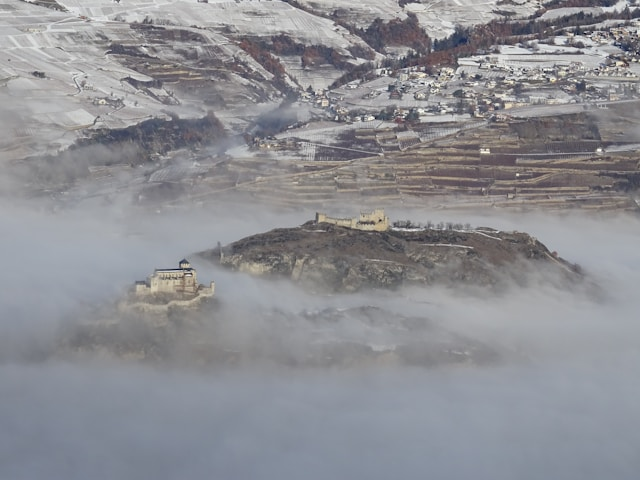
\includegraphics[width=0.9\linewidth,height=\textheight,keepaspectratio]{images/cover_matthias-kastner_sion.jpg}

}

\caption{Sion and surrounding mountains (Switzerland). Photo by Matthias
Kastner on Unsplash}

\end{figure}%

\newpage{}

\begin{tcolorbox}[enhanced jigsaw, arc=.35mm, left=2mm, toprule=.15mm, colbacktitle=quarto-callout-note-color!10!white, toptitle=1mm, breakable, opacityback=0, rightrule=.15mm, title=\textcolor{quarto-callout-note-color}{\faInfo}\hspace{0.5em}{This exercise in brief}, colframe=quarto-callout-note-color-frame, bottomrule=.15mm, colback=white, opacitybacktitle=0.6, bottomtitle=1mm, titlerule=0mm, coltitle=black, leftrule=.75mm]

\subsubsection{Big Question}\label{big-question}

Where are the areas most susceptible to new rock instabilities or
further destabilization within existing landslide zones, based on
topographic and geological factors?

\subsubsection{What You Will Do}\label{what-you-will-do}

You will combine vector geological maps with raster elevation data to
identify areas with high landslide susceptibility. Using Python
libraries developed for handling geospatial data , you will filter
specific rock types, calculate slope gradients from a Digital Elevation
Model (DEM), and apply a statistical threshold to pinpoint zones where
topography and lithology create a critical risk of failure.

\subsubsection{Why This Matters}\label{why-this-matters}

Understanding slope stability is critical for land-use planning and
hazard mitigation in Alpine environments. By analyzing the relationship
between lithology, slope angle, and historical instability ata, we can
predict future failures before they occur. This aligns with the Swiss
federal approach to hazard mapping, moving from inventory catalogs to
indicative susceptibility maps using reproducible code.

\subsubsection{Your Tasks}\label{your-tasks}

\begin{enumerate}
\def\labelenumi{\arabic{enumi}.}
\item
  \textbf{Data Filtering:} Query vector attributes to isolate
  lithologies prone to instability (Typ\_code 800, 801, 802, 870) and
  existing instability structures (Typ\_code 700, 701).
\item
  \textbf{Terrain Analysis:} Compute slope gradients from the DEM and
  calculate statistical metrics (mean) to determine the stability
  threshold (\(\phi\)).
\item
  \textbf{Susceptibility Modeling:} Apply boolean logic and raster
  masking to identify: 3.1. New potential instabilities on favorable
  lithologies where slope \textgreater{} \(\phi\). 3.2. Critical
  sub-zones within existing landslides where slope \textgreater{}
  \(\phi\).
\item
  \textbf{Visualization \& Export:} Generate static maps highlighting
  risk zones with appropriate color ramps and transparency, and export
  summary statistics (areas).
\end{enumerate}

\subsubsection{Skills You Will Gain}\label{skills-you-will-gain}

\begin{enumerate}
\def\labelenumi{\arabic{enumi}.}
\tightlist
\item
  Calculating terrain attributes (slope, hillshade) from DEM arrays.
\item
  Spatial Querying: Filtering vector data based on attribute
  expressions.
\item
  Map Algebra: Performing cell-by-cell mathematical operations and
  reclassification on raster grids.
\item
  Cartographic Output: Rendering geospatial data to image formats
  (PNG/JPG) with custom colormaps.
\end{enumerate}

\subsubsection{Points for Discussion}\label{points-for-discussion}

\begin{itemize}
\tightlist
\item
  The Threshold Assumption: We assume the mean slope of existing
  instabilities represents the internal friction angle (\(\phi\)). How
  valid is this assumption across different lithological units?
\item
  Data Resolution: How does the 25m pixel size affect the precision of
  the slope calculation and the resulting hazard boundaries?
\item
  Model Limitations: This model relies solely on slope and lithology.
  How would you integrate dynamic triggers (e.g., precipitation data,
  seismic history) into this Python workflow?
\item
  List your results (see list in the Final questions section at the
  end).
\end{itemize}

\end{tcolorbox}

\subsection{Step-by-step instructions}\label{step-by-step-instructions}

\subsubsection{Install libraries}\label{install-libraries}

This tutorial requires the following libraries:

\begin{itemize}
\tightlist
\item
  \texttt{rasterio}
\item
  \texttt{geopandas}
\item
  \texttt{matplotlib}
\item
  \texttt{numpy}
\end{itemize}

You can check if they are installed (and check which version you have)
by running:

\begin{Shaded}
\begin{Highlighting}[]
\NormalTok{libs }\OperatorTok{=}\NormalTok{ [}\StringTok{"rasterio"}\NormalTok{, }\StringTok{"geopandas"}\NormalTok{, }\StringTok{"matplotlib"}\NormalTok{, }\StringTok{"numpy"}\NormalTok{]}

\ControlFlowTok{for}\NormalTok{ lib }\KeywordTok{in}\NormalTok{ libs:}
    \ControlFlowTok{try}\NormalTok{:}
\NormalTok{        module }\OperatorTok{=} \BuiltInTok{\_\_import\_\_}\NormalTok{(lib)}
        \BuiltInTok{print}\NormalTok{(lib }\OperatorTok{+} \StringTok{" is installed"}\NormalTok{)}
    \ControlFlowTok{except} \PreprocessorTok{ImportError}\NormalTok{:}
        \BuiltInTok{print}\NormalTok{(lib }\OperatorTok{+} \StringTok{" is NOT installed"}\NormalTok{)}
\end{Highlighting}
\end{Shaded}

If you encounter an error, come back to
\href{https://unige-cgeom.github.io/SPACE-GEOLOGY/course/chapter2_setup.html}{Chapter
II: Setting up your Python environment} and follow the instructions.

\subsubsection{Data preparation}\label{data-preparation}

You are provided with the following input data:

\begin{longtable}[]{@{}
  >{\raggedright\arraybackslash}p{(\linewidth - 4\tabcolsep) * \real{0.3333}}
  >{\raggedright\arraybackslash}p{(\linewidth - 4\tabcolsep) * \real{0.3333}}
  >{\raggedright\arraybackslash}p{(\linewidth - 4\tabcolsep) * \real{0.3333}}@{}}
\toprule\noalign{}
\begin{minipage}[b]{\linewidth}\raggedright
Name
\end{minipage} & \begin{minipage}[b]{\linewidth}\raggedright
Format
\end{minipage} & \begin{minipage}[b]{\linewidth}\raggedright
Description
\end{minipage} \\
\midrule\noalign{}
\endhead
\bottomrule\noalign{}
\endlastfoot
\texttt{Sion\_MNT25.tif} & Raster & DEM of the Sion area (© Swisstopo)
at a spatial resolution of 25 m \\
\texttt{Bedrok\_PLG.shp} & Shapefile & Bedrock geology \\
\texttt{Subequil\_PLG\_r.shp} & Shapefile & Area representing a state of
sub-equilibrium. This area has been defined in the field and represents
the ground truth. \\
\end{longtable}

\paragraph{Digital elevation model}\label{digital-elevation-model}

We will first prepare our data. The first step is to load the DEM at 25m
from the Swiss Federal Office of Topography (swisstopo). The entire
dataset is described on the
\href{https://www.swisstopo.admin.ch/fr/modele-altimetrique-mnt25}{swisstopo
website}, but we will use a subset over the region of Sion, Canton of
Valais. The DEM is already provided and available in the
\href{https://github.com/unige-cgeom/SPACE-GEOLOGY/tree/main/course/data}{data}
folder as a GeoTiFF, and we open it using the
\href{https://rasterio.readthedocs.io/en/latest/api/rasterio.html\#rasterio.open}{rasterio.open}
function.

\begin{tcolorbox}[enhanced jigsaw, arc=.35mm, left=2mm, toprule=.15mm, colbacktitle=quarto-callout-note-color!10!white, toptitle=1mm, breakable, opacityback=0, rightrule=.15mm, title=\textcolor{quarto-callout-note-color}{\faInfo}\hspace{0.5em}{Question}, colframe=quarto-callout-note-color-frame, bottomrule=.15mm, colback=white, opacitybacktitle=0.6, bottomtitle=1mm, titlerule=0mm, coltitle=black, leftrule=.75mm]

Load the geotiff using \texttt{rasterio.open} as in the following block
and save the following attributes as variables:

\begin{itemize}
\tightlist
\item
  \texttt{profile}
\item
  \texttt{shape}
\item
  \texttt{bounds}
\item
  \texttt{crs}
\item
  `transform
\end{itemize}

Inspect all variables

\begin{itemize}
\tightlist
\item
  What variables are in \textbf{matrix coordinates?} What variables are
  in geographic coordinates?
\item
  What is the coordinate reference system of the layer ? What is its
  resolution ?
\end{itemize}

\end{tcolorbox}

\begin{Shaded}
\begin{Highlighting}[]
\ImportTok{import}\NormalTok{ rasterio}

\ControlFlowTok{with}\NormalTok{ rasterio.}\BuiltInTok{open}\NormalTok{(}\StringTok{"data/DEM/Sion\_MNT25.tif"}\NormalTok{) }\ImportTok{as}\NormalTok{ src:}
\NormalTok{    dem }\OperatorTok{=}\NormalTok{ src.read(}\DecValTok{1}\NormalTok{) }\CommentTok{\# The data}
\NormalTok{    profile }\OperatorTok{=}\NormalTok{ src.profile }\CommentTok{\# Raster metadata (contains all the variables below)}
\NormalTok{    shape }\OperatorTok{=}\NormalTok{ src.shape}
\NormalTok{    bounds }\OperatorTok{=}\NormalTok{ src.bounds}
\NormalTok{    crs }\OperatorTok{=}\NormalTok{ src.crs}
\NormalTok{    transform }\OperatorTok{=}\NormalTok{ src.transform }\CommentTok{\# Affine transformation}
\end{Highlighting}
\end{Shaded}

\paragraph{Lithologies favorable to rock
instabilities}\label{lithologies-favorable-to-rock-instabilities}

Second, we will extract the lithologies that favour instabilities the
\texttt{geopandas} library. This library is an extension of
\texttt{pandas} specifically designed to handle geospatial data.

You may use \texttt{geopandas} to read a \emph{vector} file (for
instance shapefile) into a \texttt{GeoDataFrame} (gdf), which is simply
a \texttt{DataFrame} that contains a geometry column. The example below
shows how to load the \texttt{Bedrok\_PLG.shp} shapefile with
\texttt{{[}gpd.read\_file{]}(https://geopandas.org/en/v1.1.0/docs/reference/api/geopandas.read\_file.html)}
and perform basic operations. Really, a \texttt{gpd} object represents
the \textbf{table of attributes} you might be familiar with in QGis.

\begin{tcolorbox}[enhanced jigsaw, arc=.35mm, left=2mm, toprule=.15mm, colbacktitle=quarto-callout-tip-color!10!white, toptitle=1mm, breakable, opacityback=0, rightrule=.15mm, title=\textcolor{quarto-callout-tip-color}{\faLightbulb}\hspace{0.5em}{Encoding}, colframe=quarto-callout-tip-color-frame, bottomrule=.15mm, colback=white, opacitybacktitle=0.6, bottomtitle=1mm, titlerule=0mm, coltitle=black, leftrule=.75mm]

Specifying the \texttt{encoding} argument to \texttt{utf-8} is critical
to preserve French accents in the attributes.

\end{tcolorbox}

\begin{Shaded}
\begin{Highlighting}[]
\ImportTok{import}\NormalTok{ geopandas }\ImportTok{as}\NormalTok{ gpd}

\NormalTok{bedrock\_plg }\OperatorTok{=}\NormalTok{ gpd.read\_file( }\VerbatimStringTok{r"data/shapefiles/Bedrok\_PLG}\DecValTok{.}\VerbatimStringTok{shp"}\NormalTok{, encoding}\OperatorTok{=}\StringTok{"utf{-}8"}
\NormalTok{)}

\CommentTok{\# Print the first 5 columns}
\NormalTok{bedrock\_plg.head(}\DecValTok{5}\NormalTok{)}

\CommentTok{\# Print the column names}
\NormalTok{bedrock\_plg.columns}

\CommentTok{\# Query the first row/feature {-} remember, in Python the first row/column is represented by the index 0 (not 1)}
\NormalTok{bedrock\_plg.iloc[}\DecValTok{0}\NormalTok{]}

\CommentTok{\# Query a specific column}
\NormalTok{bedrock\_plg[}\StringTok{\textquotesingle{}Typ\_code\textquotesingle{}}\NormalTok{]}
\end{Highlighting}
\end{Shaded}

We need to filter out the original data to keep only the lithologies of
interest. This can be done using the
\texttt{{[}pd.query(){]}(https://pandas.pydata.org/docs/reference/api/pandas.DataFrame.query.html)}
function with the desired condition:

\begin{Shaded}
\begin{Highlighting}[]
\NormalTok{select\_litho }\OperatorTok{=}\NormalTok{ bedrock\_plg.query(}\StringTok{"Typ\_code == \textquotesingle{}830\textquotesingle{}"}\NormalTok{)}
\BuiltInTok{print}\NormalTok{(select\_litho.iloc[}\DecValTok{0}\NormalTok{].Litho)}
\end{Highlighting}
\end{Shaded}

\begin{tcolorbox}[enhanced jigsaw, arc=.35mm, left=2mm, toprule=.15mm, colbacktitle=quarto-callout-tip-color!10!white, toptitle=1mm, breakable, opacityback=0, rightrule=.15mm, title=\textcolor{quarto-callout-tip-color}{\faLightbulb}\hspace{0.5em}{Pandas vs geopandas}, colframe=quarto-callout-tip-color-frame, bottomrule=.15mm, colback=white, opacitybacktitle=0.6, bottomtitle=1mm, titlerule=0mm, coltitle=black, leftrule=.75mm]

As you might notice, geopandas objects inherit from most pandas
functions, such as \texttt{query()}.

\end{tcolorbox}

\begin{tcolorbox}[enhanced jigsaw, arc=.35mm, left=2mm, toprule=.15mm, colbacktitle=quarto-callout-note-color!10!white, toptitle=1mm, breakable, opacityback=0, rightrule=.15mm, title=\textcolor{quarto-callout-note-color}{\faInfo}\hspace{0.5em}{Questions}, colframe=quarto-callout-note-color-frame, bottomrule=.15mm, colback=white, opacitybacktitle=0.6, bottomtitle=1mm, titlerule=0mm, coltitle=black, leftrule=.75mm]

\begin{itemize}
\tightlist
\item
  What lithology is associated with the code `870'?
\item
  How would you for multiple values?
\end{itemize}

\end{tcolorbox}

\begin{tcolorbox}[enhanced jigsaw, arc=.35mm, left=2mm, toprule=.15mm, colbacktitle=quarto-callout-caution-color!10!white, toptitle=1mm, breakable, opacityback=0, rightrule=.15mm, title=\textcolor{quarto-callout-caution-color}{\faFire}\hspace{0.5em}{Solutions}, colframe=quarto-callout-caution-color-frame, bottomrule=.15mm, colback=white, opacitybacktitle=0.6, bottomtitle=1mm, titlerule=0mm, coltitle=black, leftrule=.75mm]

\begin{Shaded}
\begin{Highlighting}[]
\NormalTok{fav\_litho }\OperatorTok{=}\NormalTok{ bedrock\_plg.query(}\StringTok{"Typ\_code in (\textquotesingle{}800\textquotesingle{}, \textquotesingle{}801\textquotesingle{}, \textquotesingle{}802\textquotesingle{}, \textquotesingle{}870\textquotesingle{})"}\NormalTok{)}
\BuiltInTok{print}\NormalTok{(fav\_litho.iloc[}\DecValTok{0}\NormalTok{].Litho)}
\end{Highlighting}
\end{Shaded}

\end{tcolorbox}

\subparagraph{Plotting shapefiles}\label{plotting-shapefiles}

We can easily plot the favorable lithologies, colouring each polygon
according to its `Typ\_code' attribute:

\begin{Shaded}
\begin{Highlighting}[]
\NormalTok{fav\_litho.plot(}
\NormalTok{    figsize}\OperatorTok{=}\NormalTok{(}\DecValTok{8}\NormalTok{, }\DecValTok{8}\NormalTok{),}
\NormalTok{    column}\OperatorTok{=}\StringTok{"Typ\_code"}\NormalTok{,}
\NormalTok{    legend}\OperatorTok{=}\VariableTok{True}
\NormalTok{)}
\end{Highlighting}
\end{Shaded}

\subparagraph{Converting shapefiles to
raster}\label{converting-shapefiles-to-raster}

Lithologies will be used as \textbf{mask} in the rest of the study. In
order to mask out raster data, the lithology layer needs to be converted
into a raster that is \textbf{aligned} with the raster layer to mask
(here, the \texttt{Sion\_MNT25.tif} layer). Aligned means that the
pixels of both layers have the same reference coordinates and extent,
providing a 100\% overlap. To ensure that, we use the \texttt{shape} and
\texttt{transform} variables obtained from the DEM and pass them to
\texttt{rasterio}'s
\href{https://rasterio.readthedocs.io/en/stable/api/rasterio.features.html\#rasterio.features.rasterize}{rasterize}
function:

\begin{Shaded}
\begin{Highlighting}[]
\ImportTok{from}\NormalTok{ rasterio.features }\ImportTok{import}\NormalTok{ rasterize}

\NormalTok{raster\_fav\_litho }\OperatorTok{=}\NormalTok{ rasterize(}
\NormalTok{    shapes}\OperatorTok{=}\NormalTok{((geom, }\DecValTok{1}\NormalTok{) }\ControlFlowTok{for}\NormalTok{ geom }\KeywordTok{in}\NormalTok{ fav\_litho.geometry),}
\NormalTok{    out\_shape}\OperatorTok{=}\NormalTok{shape,}
\NormalTok{    transform}\OperatorTok{=}\NormalTok{transform,}
\NormalTok{    fill}\OperatorTok{=}\DecValTok{0}\NormalTok{,}
\NormalTok{    dtype}\OperatorTok{=}\StringTok{"uint8"}
\NormalTok{)}
\end{Highlighting}
\end{Shaded}

For each polygon in the favorable lithologies, the created pixels will
have a value of 1. Other pixels will have a value of 0 (from the `fill'
parameter). Let's visualize the result:

\begin{Shaded}
\begin{Highlighting}[]
\ImportTok{import}\NormalTok{ matplotlib.pyplot }\ImportTok{as}\NormalTok{ plt}

\NormalTok{plt.imshow(raster\_fav\_litho)}
\NormalTok{plt.colorbar()}
\NormalTok{plt.axis(}\StringTok{"off"}\NormalTok{)}
\NormalTok{plt.show()}
\end{Highlighting}
\end{Shaded}

The next step is to export the raster. We ensure that the target
directory exists - or, if not, create it - using the
\href{https://docs.python.org/3/library/os.html\#os.makedirs}{makedirs}
function from the \texttt{os} library. The \texttt{os} library is used
to interact with the operating system of your machine, in this case, by
creating a folder where

\begin{Shaded}
\begin{Highlighting}[]
\ImportTok{import}\NormalTok{ os}
\NormalTok{os.makedirs(}
    \StringTok{"data/outputs"}\NormalTok{,}
\NormalTok{    exist\_ok}\OperatorTok{=}\VariableTok{True}
\NormalTok{)}

\ControlFlowTok{with}\NormalTok{ rasterio.}\BuiltInTok{open}\NormalTok{(}
    \VerbatimStringTok{r"data/outputs/fav\_litho}\DecValTok{.}\VerbatimStringTok{tif"}\NormalTok{, }\StringTok{"w"}\NormalTok{,}
\NormalTok{    driver}\OperatorTok{=}\StringTok{"GTiff"}\NormalTok{,}
\NormalTok{    height}\OperatorTok{=}\NormalTok{shape[}\DecValTok{0}\NormalTok{], width}\OperatorTok{=}\NormalTok{shape[}\DecValTok{1}\NormalTok{],}
\NormalTok{    count}\OperatorTok{=}\DecValTok{1}\NormalTok{, dtype}\OperatorTok{=}\StringTok{"uint8"}\NormalTok{,}
\NormalTok{    crs}\OperatorTok{=}\NormalTok{crs, transform}\OperatorTok{=}\NormalTok{transform}
\NormalTok{) }\ImportTok{as}\NormalTok{ dst:}
\NormalTok{    dst.write(raster\_fav\_litho, }\DecValTok{1}\NormalTok{)}
\end{Highlighting}
\end{Shaded}

The code writes a \texttt{GeoTiFF} file with the same properties (shape,
crs, transform) as the original DEM, with one band (defined by the
`count' parameter).

→ Let's go back to our rasterized favorable lithologies. Try calculating
the area covered by such lithologies. This can be done by multiplying
the raster pixels width, height and count. The first two are available
in the \texttt{transform} property of the raster metadata (originally
from the DEM, that we also applied to our rasterized lithologies). The
pixel count can be obtained using \texttt{numpy} summing operations.

\begin{Shaded}
\begin{Highlighting}[]
\ImportTok{import}\NormalTok{ numpy }\ImportTok{as}\NormalTok{ np}
\NormalTok{pixel\_width }\OperatorTok{=} \BuiltInTok{abs}\NormalTok{(transform[}\DecValTok{0}\NormalTok{])}
\NormalTok{pixel\_height }\OperatorTok{=} \BuiltInTok{abs}\NormalTok{(transform[}\DecValTok{4}\NormalTok{])}
\NormalTok{pixel\_area }\OperatorTok{=}\NormalTok{ pixel\_width }\OperatorTok{*}\NormalTok{ pixel\_height}

\NormalTok{pixel\_count }\OperatorTok{=}\NormalTok{ np.}\BuiltInTok{sum}\NormalTok{(raster\_fav\_litho }\OperatorTok{==} \DecValTok{1}\NormalTok{)}

\NormalTok{total\_area }\OperatorTok{=}\NormalTok{ pixel\_count }\OperatorTok{*}\NormalTok{ pixel\_area}
\BuiltInTok{print}\NormalTok{(total\_area)}
\end{Highlighting}
\end{Shaded}

→ What does this number represent ? What units ?

\paragraph{Existing instabilities}\label{existing-instabilities}

Ler's now inspect and identify existing rock instabilities. Load the
`Instability\_Structures\_PLG' shapefile and inspect its features in a
similar fashion than for the bedrock polygons.

\begin{tcolorbox}[enhanced jigsaw, arc=.35mm, left=2mm, toprule=.15mm, colbacktitle=quarto-callout-tip-color!10!white, toptitle=1mm, breakable, opacityback=0, rightrule=.15mm, title=\textcolor{quarto-callout-tip-color}{\faLightbulb}\hspace{0.5em}{Unique values}, colframe=quarto-callout-tip-color-frame, bottomrule=.15mm, colback=white, opacitybacktitle=0.6, bottomtitle=1mm, titlerule=0mm, coltitle=black, leftrule=.75mm]

You can display all \emph{unique values} in one column using
\texttt{df{[}\textquotesingle{}col\_name\textquotesingle{}{]}.unique()}.

\end{tcolorbox}

\begin{Shaded}
\begin{Highlighting}[]
\NormalTok{instabilities\_plg }\OperatorTok{=}\NormalTok{ gpd.read\_file(}
    \VerbatimStringTok{r"data/shapefiles/Instability\_Structures\_PLG}\DecValTok{.}\VerbatimStringTok{shp"}\NormalTok{,}
\NormalTok{    encoding}\OperatorTok{=}\StringTok{"utf{-}8"}
\NormalTok{)}

\CommentTok{\# Print the columns}
\BuiltInTok{print}\NormalTok{(instabilities\_plg.columns)}
\CommentTok{\# Print the first 10 rows}
\BuiltInTok{print}\NormalTok{(instabilities\_plg.head(}\DecValTok{10}\NormalTok{))}

\BuiltInTok{print}\NormalTok{(}\StringTok{"First feature:"}\NormalTok{,instabilities\_plg.iloc[}\DecValTok{0}\NormalTok{])}

\BuiltInTok{print}\NormalTok{(}\StringTok{"First feature geometry:"}\NormalTok{,instabilities\_plg.iloc[}\DecValTok{0}\NormalTok{].geometry)}

\NormalTok{instabilities\_plg[}\StringTok{"TYP\_CODE"}\NormalTok{].unique()}
\NormalTok{instabilities\_plg[}\StringTok{"TYP\_NAME"}\NormalTok{].unique()}
\end{Highlighting}
\end{Shaded}

→ What are the instabilities you identified?

→ Try plotting the polygons of instabilities with a symbology based on
the type

Let's now filter out our existing instabilities using the codes we found
in the previous code, and calculate their combined area.

\begin{Shaded}
\begin{Highlighting}[]
\NormalTok{existing\_instabilities }\OperatorTok{=}\NormalTok{ instabilities\_plg.query(}\StringTok{"TYP\_CODE in (\textquotesingle{}700\textquotesingle{}, \textquotesingle{}701\textquotesingle{})"}\NormalTok{)}
\NormalTok{existing\_instabilities[}\StringTok{"area\_m2"}\NormalTok{] }\OperatorTok{=}\NormalTok{ existing\_instabilities.geometry.area}

\NormalTok{total\_area\_plg }\OperatorTok{=}\NormalTok{ existing\_instabilities.geometry.area.}\BuiltInTok{sum}\NormalTok{()}

\BuiltInTok{print}\NormalTok{(}\SpecialStringTok{f"Total area from polygons: }\SpecialCharTok{\{}\NormalTok{total\_area\_plg}\SpecialCharTok{\}}\SpecialStringTok{"}\NormalTok{)}
\end{Highlighting}
\end{Shaded}

Notice how we were able to calculate the area directly on the vector
data, unlike what we did with the favorable lithologies ?

→ Both methods are possible, but which one do you think is best suited ?
Why ?

→ Rasterize the existing instabilities and calculate the area on the
pixels. What result do you get ?

\begin{Shaded}
\begin{Highlighting}[]
\NormalTok{raster\_inst }\OperatorTok{=}\NormalTok{ rasterize(}
\NormalTok{    shapes}\OperatorTok{=}\NormalTok{((geom, }\DecValTok{1}\NormalTok{) }\ControlFlowTok{for}\NormalTok{ geom }\KeywordTok{in}\NormalTok{ existing\_instabilities.geometry),}
\NormalTok{    out\_shape}\OperatorTok{=}\NormalTok{shape,}
\NormalTok{    transform}\OperatorTok{=}\NormalTok{transform,}
\NormalTok{    fill}\OperatorTok{=}\DecValTok{0}\NormalTok{,}
\NormalTok{    dtype}\OperatorTok{=}\StringTok{"uint8"}
\NormalTok{)}

\NormalTok{pixel\_count }\OperatorTok{=}\NormalTok{ np.}\BuiltInTok{sum}\NormalTok{(raster\_inst }\OperatorTok{==} \DecValTok{1}\NormalTok{)}

\NormalTok{total\_area }\OperatorTok{=}\NormalTok{ pixel\_count }\OperatorTok{*}\NormalTok{ pixel\_area}
\BuiltInTok{print}\NormalTok{(}\SpecialStringTok{f"Total area from pixels: }\SpecialCharTok{\{}\NormalTok{total\_area}\SpecialCharTok{\}}\SpecialStringTok{"}\NormalTok{)}
\end{Highlighting}
\end{Shaded}

Let's also export our data to a GeoTiFF using the same command as
before.

\begin{Shaded}
\begin{Highlighting}[]
\ControlFlowTok{with}\NormalTok{ rasterio.}\BuiltInTok{open}\NormalTok{(}
    \VerbatimStringTok{r"data/outputs/instabilities}\DecValTok{.}\VerbatimStringTok{tif"}\NormalTok{, }\StringTok{"w"}\NormalTok{,}
\NormalTok{    driver}\OperatorTok{=}\StringTok{"GTiff"}\NormalTok{,}
\NormalTok{    height}\OperatorTok{=}\NormalTok{shape[}\DecValTok{0}\NormalTok{], width}\OperatorTok{=}\NormalTok{shape[}\DecValTok{1}\NormalTok{],}
\NormalTok{    count}\OperatorTok{=}\DecValTok{1}\NormalTok{, dtype}\OperatorTok{=}\StringTok{"uint8"}\NormalTok{,}
\NormalTok{    crs}\OperatorTok{=}\NormalTok{crs, transform}\OperatorTok{=}\NormalTok{transform}
\NormalTok{) }\ImportTok{as}\NormalTok{ dst:}
\NormalTok{    dst.write(raster\_inst, }\DecValTok{1}\NormalTok{)}
\end{Highlighting}
\end{Shaded}

\paragraph{Slope distribution}\label{slope-distribution}

We are going to calculate the slope of each pixel from the original DEM
to understand the terrain variations and how these are related to
instabilities. In traditional Desktop GIS, there are some tools that
already implement slope calculations, but we can do it manually using
\texttt{numpy} in Python, se we understand how the slope is calculated.

The slope of a cell is usually calculated using the Horn algorithm
(Horn, 1981), and considers the 8 neighbouring cells elevation (N, S, E,
W, NE, NW, SE, SW). With \texttt{np.roll}, we can retrieve the
information about each neighbouring cell by just shifting the array, for
every cell at once.

\begin{Shaded}
\begin{Highlighting}[]
\NormalTok{north }\OperatorTok{=}\NormalTok{ np.roll(dem, }\OperatorTok{{-}}\DecValTok{1}\NormalTok{, axis}\OperatorTok{=}\DecValTok{0}\NormalTok{)}
\NormalTok{south }\OperatorTok{=}\NormalTok{ np.roll(dem,  }\DecValTok{1}\NormalTok{, axis}\OperatorTok{=}\DecValTok{0}\NormalTok{)}
\NormalTok{east }\OperatorTok{=}\NormalTok{ np.roll(dem,  }\DecValTok{1}\NormalTok{, axis}\OperatorTok{=}\DecValTok{1}\NormalTok{)}
\NormalTok{west }\OperatorTok{=}\NormalTok{ np.roll(dem, }\OperatorTok{{-}}\DecValTok{1}\NormalTok{, axis}\OperatorTok{=}\DecValTok{1}\NormalTok{)}

\NormalTok{north\_east }\OperatorTok{=}\NormalTok{ np.roll(north,  }\DecValTok{1}\NormalTok{, axis}\OperatorTok{=}\DecValTok{1}\NormalTok{)}
\NormalTok{north\_west }\OperatorTok{=}\NormalTok{ np.roll(north, }\OperatorTok{{-}}\DecValTok{1}\NormalTok{, axis}\OperatorTok{=}\DecValTok{1}\NormalTok{)}
\NormalTok{south\_east }\OperatorTok{=}\NormalTok{ np.roll(south,  }\DecValTok{1}\NormalTok{, axis}\OperatorTok{=}\DecValTok{1}\NormalTok{)}
\NormalTok{south\_west }\OperatorTok{=}\NormalTok{ np.roll(south, }\OperatorTok{{-}}\DecValTok{1}\NormalTok{, axis}\OperatorTok{=}\DecValTok{1}\NormalTok{)}
\end{Highlighting}
\end{Shaded}

Then, using Horn's formula, we calculate how much elevation changes
east-west (dx) and north-south (dy), that will help us calculate the
slope in degrees.

\begin{Shaded}
\begin{Highlighting}[]
\NormalTok{dx }\OperatorTok{=}\NormalTok{ ((north\_east }\OperatorTok{+} \DecValTok{2}\OperatorTok{*}\NormalTok{east }\OperatorTok{+}\NormalTok{ south\_east }\OperatorTok{{-}}\NormalTok{ north\_west }\OperatorTok{{-}} \DecValTok{2}\OperatorTok{*}\NormalTok{west }\OperatorTok{{-}}\NormalTok{ south\_west)}
      \OperatorTok{/}\NormalTok{ (}\DecValTok{8} \OperatorTok{*}\NormalTok{ pixel\_width))}
\NormalTok{dy }\OperatorTok{=}\NormalTok{ ((south\_west }\OperatorTok{+} \DecValTok{2}\OperatorTok{*}\NormalTok{south }\OperatorTok{+}\NormalTok{ south\_east }\OperatorTok{{-}}\NormalTok{ north\_west }\OperatorTok{{-}} \DecValTok{2}\OperatorTok{*}\NormalTok{north }\OperatorTok{{-}}\NormalTok{ north\_east)}
      \OperatorTok{/}\NormalTok{ (}\DecValTok{8} \OperatorTok{*}\NormalTok{ pixel\_height))}

\NormalTok{slope\_deg }\OperatorTok{=}\NormalTok{ np.degrees(np.arctan(np.sqrt(dx}\OperatorTok{**}\DecValTok{2} \OperatorTok{+}\NormalTok{ dy}\OperatorTok{**}\DecValTok{2}\NormalTok{)))}
\end{Highlighting}
\end{Shaded}

Note that all operations, including \texttt{np.roll},
\texttt{np.degrees} or \texttt{np.arctan} are performed on every pixel
of the DEM, this is what we call vectorized operations. It is built-in
to work faster and in a cleaner way than what a loop would do.

Before moving on to analyze our slope values, we need to correct for the
issue with slope calculation at the map's edges. When we do
\texttt{np.roll}, the pixels of the first and last rows, together with
pixels from the first and last column are moved to the other end of the
raster and might induce errors locally. For this reason, we will discard
them from our analysis by assigning them the `not a number' (NaN) value.

\begin{Shaded}
\begin{Highlighting}[]
\NormalTok{slope\_deg[}\DecValTok{0}\NormalTok{, :]  }\OperatorTok{=}\NormalTok{ np.nan}
\NormalTok{slope\_deg[}\OperatorTok{{-}}\DecValTok{1}\NormalTok{, :] }\OperatorTok{=}\NormalTok{ np.nan}
\NormalTok{slope\_deg[:, }\DecValTok{0}\NormalTok{]  }\OperatorTok{=}\NormalTok{ np.nan}
\NormalTok{slope\_deg[:, }\OperatorTok{{-}}\DecValTok{1}\NormalTok{] }\OperatorTok{=}\NormalTok{ np.nan}
\end{Highlighting}
\end{Shaded}

In the code above, we simply take all pixels from the first row
\texttt{{[}0,:{]}}, all pixels from the last row {[}-1,:{]}, all pixels
form the first column \texttt{{[}:,0{]}} and all pixels from the last
column \texttt{{[}:,-1{]}} and set them to NaN using \texttt{np.nan}

Let's now have a look at our values and print the minimum, maximum and
mean slope.

\begin{Shaded}
\begin{Highlighting}[]
\BuiltInTok{print}\NormalTok{(}\SpecialStringTok{f"Min slope:  }\SpecialCharTok{\{}\NormalTok{np}\SpecialCharTok{.}\NormalTok{nanmin(slope\_deg)}\SpecialCharTok{\}}\SpecialStringTok{°"}\NormalTok{)}
\BuiltInTok{print}\NormalTok{(}\SpecialStringTok{f"Max slope:  }\SpecialCharTok{\{}\NormalTok{np}\SpecialCharTok{.}\NormalTok{nanmax(slope\_deg)}\SpecialCharTok{\}}\SpecialStringTok{°"}\NormalTok{)}
\BuiltInTok{print}\NormalTok{(}\SpecialStringTok{f"Mean slope: }\SpecialCharTok{\{}\NormalTok{np}\SpecialCharTok{.}\NormalTok{nanmean(slope\_deg)}\SpecialCharTok{\}}\SpecialStringTok{°"}\NormalTok{)}
\end{Highlighting}
\end{Shaded}

→ Plot and save the slope map !

\begin{Shaded}
\begin{Highlighting}[]
\NormalTok{left }\OperatorTok{=}\NormalTok{ transform[}\DecValTok{2}\NormalTok{]}
\NormalTok{right }\OperatorTok{=}\NormalTok{ transform[}\DecValTok{2}\NormalTok{] }\OperatorTok{+}\NormalTok{ transform[}\DecValTok{0}\NormalTok{] }\OperatorTok{*}\NormalTok{ dem.shape[}\DecValTok{1}\NormalTok{]}
\NormalTok{bottom }\OperatorTok{=}\NormalTok{ transform[}\DecValTok{5}\NormalTok{] }\OperatorTok{+}\NormalTok{ transform[}\DecValTok{4}\NormalTok{] }\OperatorTok{*}\NormalTok{ dem.shape[}\DecValTok{0}\NormalTok{]}
\NormalTok{top }\OperatorTok{=}\NormalTok{ transform[}\DecValTok{5}\NormalTok{]}

\NormalTok{plt.figure(figsize}\OperatorTok{=}\NormalTok{(}\DecValTok{8}\NormalTok{, }\DecValTok{8}\NormalTok{))}
\NormalTok{plt.imshow(}
\NormalTok{    slope\_deg,}
\NormalTok{    cmap}\OperatorTok{=}\StringTok{"magma"}\NormalTok{,}
\NormalTok{    extent}\OperatorTok{=}\NormalTok{[left, right, bottom, top]}
\NormalTok{)}
\NormalTok{plt.colorbar(label}\OperatorTok{=}\StringTok{"Slope (degrees)"}\NormalTok{)}
\NormalTok{plt.show()}

\ControlFlowTok{with}\NormalTok{ rasterio.}\BuiltInTok{open}\NormalTok{(}
    \StringTok{"data/outputs/slope.tif"}\NormalTok{,}
    \StringTok{"w"}\NormalTok{,}
\NormalTok{    driver}\OperatorTok{=}\StringTok{"GTiff"}\NormalTok{,}
\NormalTok{    height}\OperatorTok{=}\NormalTok{shape[}\DecValTok{0}\NormalTok{],}
\NormalTok{    width}\OperatorTok{=}\NormalTok{shape[}\DecValTok{1}\NormalTok{],}
\NormalTok{    count}\OperatorTok{=}\DecValTok{1}\NormalTok{,}
\NormalTok{    dtype}\OperatorTok{=}\StringTok{"float32"}\NormalTok{,}
\NormalTok{    crs}\OperatorTok{=}\NormalTok{crs,}
\NormalTok{    transform}\OperatorTok{=}\NormalTok{transform,}
\NormalTok{    nodata}\OperatorTok{=}\NormalTok{np.nan}
\NormalTok{) }\ImportTok{as}\NormalTok{ dst:}
\NormalTok{    dst.write(slope\_deg.astype(}\StringTok{"float32"}\NormalTok{), }\DecValTok{1}\NormalTok{)}
\end{Highlighting}
\end{Shaded}

→ Do you understand how we calculated the extent of the map (left,
right, bottom, top) ?

\begin{tcolorbox}[enhanced jigsaw, arc=.35mm, left=2mm, toprule=.15mm, colbacktitle=quarto-callout-tip-color!10!white, toptitle=1mm, breakable, opacityback=0, rightrule=.15mm, title=\textcolor{quarto-callout-tip-color}{\faLightbulb}\hspace{0.5em}{Python libraries}, colframe=quarto-callout-tip-color-frame, bottomrule=.15mm, colback=white, opacitybacktitle=0.6, bottomtitle=1mm, titlerule=0mm, coltitle=black, leftrule=.75mm]

The advantage of open-source software is the wealth of available tools
developed by and available for the community. The method shown above
illustrates how to code an algorithm for slope computation for scratch.
However, other libraries specifically designed for DEM handling provide
numerous functions for terrain analyses (e.g.,
\href{https://github.com/creare-com/pydem}{PyDEM}), including slope,
aspects, curvature etc\ldots{}

\end{tcolorbox}

\subsubsection{Estimate the representative slope
angle}\label{estimate-the-representative-slope-angle}

Let's now have a look at a specific zone in which we observe
instabilities. The area is defined by the polygon
`subequil\_PLG\_r.shp'. We will load the shapefile and have a look at
the slope values inside this very polygon.

To do this, we will use the \texttt{geometry\_mask} function from
\texttt{rasterio}. Remember, we used masks in our first exercise by
selecting pixels above sea level, but here we will select all pixels of
the slope layer inside the sub-equilibrium polygon.

\begin{Shaded}
\begin{Highlighting}[]
\ImportTok{from}\NormalTok{ rasterio.features }\ImportTok{import}\NormalTok{ geometry\_mask}

\NormalTok{subequil\_zone }\OperatorTok{=}\NormalTok{ gpd.read\_file(}\StringTok{"data/shapefiles/subequil\_PLG\_r.shp"}\NormalTok{)}

\NormalTok{mask }\OperatorTok{=}\NormalTok{ geometry\_mask(}
\NormalTok{    subequil\_zone.geometry,}
\NormalTok{    transform}\OperatorTok{=}\NormalTok{transform,}
\NormalTok{    invert}\OperatorTok{=}\VariableTok{True}\NormalTok{,}
\NormalTok{    out\_shape}\OperatorTok{=}\NormalTok{shape}
\NormalTok{)}

\NormalTok{slope\_inside }\OperatorTok{=}\NormalTok{ slope\_deg[mask]}

\BuiltInTok{print}\NormalTok{(}\SpecialStringTok{f"Mean slope inside zone: }\SpecialCharTok{\{}\NormalTok{np}\SpecialCharTok{.}\NormalTok{nanmean(slope\_inside)}\SpecialCharTok{:.2f\}}\SpecialStringTok{°"}\NormalTok{)}
\BuiltInTok{print}\NormalTok{(}\SpecialStringTok{f"Max slope inside zone:  }\SpecialCharTok{\{}\NormalTok{np}\SpecialCharTok{.}\NormalTok{nanmax(slope\_inside)}\SpecialCharTok{:.2f\}}\SpecialStringTok{°"}\NormalTok{)}
\end{Highlighting}
\end{Shaded}

→ Plot an histogram that shows the slope distribution within the
sampling zone.

\begin{Shaded}
\begin{Highlighting}[]
\NormalTok{mean\_slope }\OperatorTok{=}\NormalTok{ np.mean(slope\_inside)}

\NormalTok{plt.hist(}
\NormalTok{    slope\_inside,}
\NormalTok{    bins}\OperatorTok{=}\DecValTok{50}
\NormalTok{)}
\NormalTok{plt.axvline(}
\NormalTok{    mean\_slope,}
\NormalTok{    color}\OperatorTok{=}\StringTok{\textquotesingle{}red\textquotesingle{}}\NormalTok{,}
\NormalTok{    linestyle}\OperatorTok{=}\StringTok{\textquotesingle{}{-}{-}\textquotesingle{}}\NormalTok{,}
\NormalTok{    label}\OperatorTok{=}\SpecialStringTok{f\textquotesingle{}Mean: }\SpecialCharTok{\{}\NormalTok{mean\_slope}\SpecialCharTok{\}}\SpecialStringTok{°\textquotesingle{}}\NormalTok{)}
\NormalTok{plt.xlabel(}\StringTok{"Slope (°)"}\NormalTok{)}
\NormalTok{plt.title(}\StringTok{"Slope distribution inside zone"}\NormalTok{)}
\NormalTok{plt.legend()}
\NormalTok{plt.show()}
\end{Highlighting}
\end{Shaded}

\subsubsection{Identify new areas susceptible to
instabilities}\label{identify-new-areas-susceptible-to-instabilities}

\paragraph{Existing instabilities on favorable
lithologies}\label{existing-instabilities-on-favorable-lithologies}

Now, we will identify areas where we have existing instabilities at
locations where the lithology is favorable.

→ Create a new raster (with the same resolution as the original DEM) to
identify existing instabilities located on favorable lithologies.

\begin{Shaded}
\begin{Highlighting}[]
\NormalTok{instabilities\_on\_fav\_litho }\OperatorTok{=}\NormalTok{ raster\_fav\_litho }\OperatorTok{*}\NormalTok{ raster\_inst}
\end{Highlighting}
\end{Shaded}

→ Plot the new raster and calculate its area

\begin{Shaded}
\begin{Highlighting}[]
\NormalTok{plt.imshow(instabilities\_on\_fav\_litho)}
\NormalTok{plt.colorbar()}
\NormalTok{plt.axis(}\StringTok{"off"}\NormalTok{)}
\NormalTok{plt.title(}\StringTok{"Existing instabilities on favorable lithologies"}\NormalTok{)}
\NormalTok{plt.show()}

\NormalTok{pixel\_count }\OperatorTok{=}\NormalTok{ np.}\BuiltInTok{sum}\NormalTok{(instabilities\_on\_fav\_litho }\OperatorTok{==} \DecValTok{1}\NormalTok{)}
\BuiltInTok{print}\NormalTok{(}
    \SpecialStringTok{f"Area of existing instabilities on favorable lithologies: "}
    \SpecialStringTok{f"}\SpecialCharTok{\{}\NormalTok{pixel\_count }\OperatorTok{*}\NormalTok{ pixel\_area}\SpecialCharTok{:.0f\}}\SpecialStringTok{ m²"}
\NormalTok{)}
\end{Highlighting}
\end{Shaded}

\paragraph{Zones without instabilities but located on favorable
lithologies}\label{zones-without-instabilities-but-located-on-favorable-lithologies}

→Using a similar approach, identify the areas where we have favorable
lithologies but no observed instabilities.

\begin{Shaded}
\begin{Highlighting}[]
\NormalTok{fav\_litho\_no\_instability }\OperatorTok{=}\NormalTok{ (raster\_fav\_litho }\OperatorTok{==} \DecValTok{1}\NormalTok{) }\OperatorTok{\&}\NormalTok{ (raster\_inst }\OperatorTok{==} \DecValTok{0}\NormalTok{)}

\NormalTok{pixel\_count }\OperatorTok{=}\NormalTok{ np.}\BuiltInTok{sum}\NormalTok{(fav\_litho\_no\_instability)}
\BuiltInTok{print}\NormalTok{(}
    \SpecialStringTok{f"Area without instabilities but with favorable lithologies: "}
    \SpecialStringTok{f"}\SpecialCharTok{\{}\NormalTok{pixel\_count }\OperatorTok{*}\NormalTok{ pixel\_area}\SpecialCharTok{\}}\SpecialStringTok{ m²"}
\NormalTok{)}
\end{Highlighting}
\end{Shaded}

\paragraph{Slopes of zone without instabilities but with favorable
lithologies}\label{slopes-of-zone-without-instabilities-but-with-favorable-lithologies}

We will now create a subset of our slope map, focusing only on the zones
where we have no instabilities and with favorable lithologies.

\begin{Shaded}
\begin{Highlighting}[]
\NormalTok{slope\_fav\_no\_inst }\OperatorTok{=}\NormalTok{ slope\_deg[fav\_litho\_no\_instability]}
\NormalTok{slope\_fav\_no\_inst }\OperatorTok{=}\NormalTok{ slope\_fav\_no\_inst[np.isfinite(slope\_fav\_no\_inst)]}
\BuiltInTok{print}\NormalTok{(}\SpecialStringTok{f"Min slope: }\SpecialCharTok{\{}\NormalTok{np}\SpecialCharTok{.}\NormalTok{nanmin(slope\_fav\_no\_inst)}\SpecialCharTok{\}}\SpecialStringTok{°"}\NormalTok{)}
\BuiltInTok{print}\NormalTok{(}\SpecialStringTok{f"Max slope:  }\SpecialCharTok{\{}\NormalTok{np}\SpecialCharTok{.}\NormalTok{nanmax(slope\_fav\_no\_inst)}\SpecialCharTok{\}}\SpecialStringTok{°"}\NormalTok{)}
\end{Highlighting}
\end{Shaded}

Given that we have all slope values over our area of interest, we will
keep only pixels that have a slope higher than the \(\phi\) value we
calculated in the part 2 above. This will give us areas susceptible to
instabilities.

→ To do this, reclassify our subset slope raster into two classes,
depending on the value of the slope value versus the \(\phi\) value.

\begin{Shaded}
\begin{Highlighting}[]
\NormalTok{slope\_class }\OperatorTok{=}\NormalTok{ np.where(slope\_deg }\OperatorTok{\textgreater{}}\NormalTok{ mean\_slope, }\DecValTok{1}\NormalTok{, }\DecValTok{0}\NormalTok{)}
\NormalTok{susceptible\_inst }\OperatorTok{=}\NormalTok{ slope\_class }\OperatorTok{*}\NormalTok{ fav\_litho\_no\_instability}

\NormalTok{pixel\_count }\OperatorTok{=}\NormalTok{ np.}\BuiltInTok{sum}\NormalTok{(susceptible\_inst }\OperatorTok{==} \DecValTok{1}\NormalTok{)}
\BuiltInTok{print}\NormalTok{(}\SpecialStringTok{f"Area susceptible to instabilities: }\SpecialCharTok{\{}\NormalTok{pixel\_count }\OperatorTok{*}\NormalTok{ pixel\_area}\SpecialCharTok{:.0f\}}\SpecialStringTok{ m²"}\NormalTok{)}
\end{Highlighting}
\end{Shaded}

\subsubsection{Susceptible areas inside the existing instability
zones}\label{susceptible-areas-inside-the-existing-instability-zones}

→ Repeat the slope subset over existing instabilities (`raster\_inst')
and calculate the area where the slope is greater than \(\phi\).

\begin{Shaded}
\begin{Highlighting}[]
\NormalTok{slope\_inst }\OperatorTok{=}\NormalTok{ slope\_deg[raster\_inst]}
\NormalTok{slope\_inst }\OperatorTok{=}\NormalTok{ slope\_inst[np.isfinite(slope\_inst)]}
\BuiltInTok{print}\NormalTok{(}\SpecialStringTok{f"Min slope: }\SpecialCharTok{\{}\NormalTok{np}\SpecialCharTok{.}\NormalTok{nanmin(slope\_inst)}\SpecialCharTok{\}}\SpecialStringTok{°"}\NormalTok{)}
\BuiltInTok{print}\NormalTok{(}\SpecialStringTok{f"Max slope:  }\SpecialCharTok{\{}\NormalTok{np}\SpecialCharTok{.}\NormalTok{nanmax(slope\_inst)}\SpecialCharTok{\}}\SpecialStringTok{°"}\NormalTok{)}

\NormalTok{slope\_class }\OperatorTok{=}\NormalTok{ np.where(slope\_deg }\OperatorTok{\textgreater{}}\NormalTok{ mean\_slope, }\DecValTok{1}\NormalTok{, }\DecValTok{0}\NormalTok{)}
\NormalTok{exist\_inst\_class }\OperatorTok{=}\NormalTok{ slope\_class }\OperatorTok{*}\NormalTok{ raster\_inst}

\NormalTok{pixel\_count }\OperatorTok{=}\NormalTok{ np.}\BuiltInTok{sum}\NormalTok{(exist\_inst\_class }\OperatorTok{==} \DecValTok{1}\NormalTok{)}
\BuiltInTok{print}\NormalTok{(}\SpecialStringTok{f"Area of existing risk: }\SpecialCharTok{\{}\NormalTok{pixel\_count }\OperatorTok{*}\NormalTok{ pixel\_area}\SpecialCharTok{\}}\SpecialStringTok{ m²"}\NormalTok{)}
\end{Highlighting}
\end{Shaded}

\subsubsection{Total susceptible areas to rock
instabilities}\label{total-susceptible-areas-to-rock-instabilities}

→ Using all of the results you obtained, calculate the total area where
we have a susceptibility to instabilities.

\begin{Shaded}
\begin{Highlighting}[]
\NormalTok{total\_susceptible }\OperatorTok{=}\NormalTok{ susceptible\_inst }\OperatorTok{+}\NormalTok{ exist\_inst\_class}
\NormalTok{total\_susceptible }\OperatorTok{=}\NormalTok{ (total\_susceptible }\OperatorTok{\textgreater{}=} \DecValTok{1}\NormalTok{).astype(}\StringTok{"uint8"}\NormalTok{)}

\NormalTok{pixel\_count }\OperatorTok{=}\NormalTok{ np.}\BuiltInTok{sum}\NormalTok{(total\_susceptible }\OperatorTok{==} \DecValTok{1}\NormalTok{)}
\BuiltInTok{print}\NormalTok{(}\SpecialStringTok{f"Total susceptible area: }\SpecialCharTok{\{}\NormalTok{pixel\_count }\OperatorTok{*}\NormalTok{ pixel\_area}\SpecialCharTok{:.0f\}}\SpecialStringTok{ m²"}\NormalTok{)}


\BuiltInTok{print}\NormalTok{(}
    \SpecialStringTok{f"New potential instabilities (fav. litho, no existing instability): "}
    \SpecialStringTok{f"}\SpecialCharTok{\{}\NormalTok{np}\SpecialCharTok{.}\BuiltInTok{sum}\NormalTok{(susceptible\_inst }\OperatorTok{==} \DecValTok{1}\NormalTok{) }\OperatorTok{*}\NormalTok{ pixel\_area}\SpecialCharTok{\}}\SpecialStringTok{ m²"}
\NormalTok{)}
\BuiltInTok{print}\NormalTok{(}
    \SpecialStringTok{f"Critical zones within existing instabilities:"}
    \SpecialStringTok{f"}\SpecialCharTok{\{}\NormalTok{np}\SpecialCharTok{.}\BuiltInTok{sum}\NormalTok{(exist\_inst\_class }\OperatorTok{==} \DecValTok{1}\NormalTok{) }\OperatorTok{*}\NormalTok{ pixel\_area}\SpecialCharTok{\}}\SpecialStringTok{ m²"}
\NormalTok{)}
\end{Highlighting}
\end{Shaded}

\subsection{Final questions}\label{final-questions}

\begin{itemize}
\tightlist
\item
  The Threshold Assumption: We assume the mean slope of existing
  instabilities represents the internal friction angle (\(\phi\)). How
  valid is this assumption across different lithological units?
\item
  Data Resolution: How does the 25m pixel size affect the precision of
  the slope calculation and the resulting hazard boundaries?
\item
  Model Limitations: This model relies solely on slope and lithology.
  How would you integrate dynamic triggers (e.g., precipitation data,
  seismic history) into this Python workflow?
\item
  List your results:

  \begin{itemize}
  \tightlist
  \item
    What proportion (in \%) of the area of the favorable lithologies is
    currently instable ? Provide all the necessary numbers used for the
    calculation.
  \item
    What proportion (in \%) of the zones situated on favorable
    lithologies could be more likely destabilized in the future? Provide
    all the necessary numbers used for the calculation.
  \item
    What proportion (in \%) of the study area is affected by
    instabilities ? Provide all the necessary numbers used for the
    calculation.
  \item
    What proportion (in \%) of the area of the existing instabilities is
    susceptible to new instabilities. Provide all the necessary numbers
    used for the calculation.
  \item
    What proportion (in \%) of the study area is still susceptible to
    instabilities? Provide all the necessary numbers used for the
    calculation.
  \end{itemize}
\end{itemize}

\subsection{Links to useful libraries and
tools}\label{links-to-useful-libraries-and-tools}

\subsubsection{Python libraries}\label{python-libraries-1}

\begin{itemize}
\item
  \href{https://geopandas.org/}{\texttt{geopandas}} An extension of
  pandas for working with geospatial vector data, adding geometry
  support and spatial operations to DataFrames.
\item
  \href{https://docs.python.org/3/library/os.html}{\texttt{os}} A Python
  standard library module for interacting with the operating system,
  including file and directory management.
\end{itemize}




\end{document}
